% !TeX root = ../main.tex
\chapter{基于高质量图像分类数据扩展的预训练方法}
\label{cha:iclip}
\label{sec:iclip-intro}
语言-图像对比学习方法通过对比学习框架在图文对数据中寻找正负样本对进行训练。其中图像及对应替代文本构成正样本对,该图像与其他替代文本构成负样本对。互联网数据中的替代文本来源多样,包含丰富的语义信息,使模型能够学习文本中的类别和属性与图像的关联关系,从而具备零样本开放集合图像识别能力。
然而,如图\ref{fig:iclip-overall}左侧所示,自动爬取的互联网图文对数据没有经过额外的人工标注或校对,往往包含图文无关的噪声(如相机参数、推广信息等),以及关联关系模糊、区分性不强的图文对数据。这些噪声数据会影响视觉表征对语义概念的建模效果,降低表征的判别能力。一般基于图像分辨率、文本长度过滤的启发式规则\cite{sharma-etal-2018-conceptual,changpinyo2021conceptual}比较简单,无法有效去除语义层面的噪声。因此,扩展高质量数据源并降低数据噪声的影响,是提升CLIP方法预训练效果的重要方向,也是本章的研究目标。

\begin{figure}
  \centering
  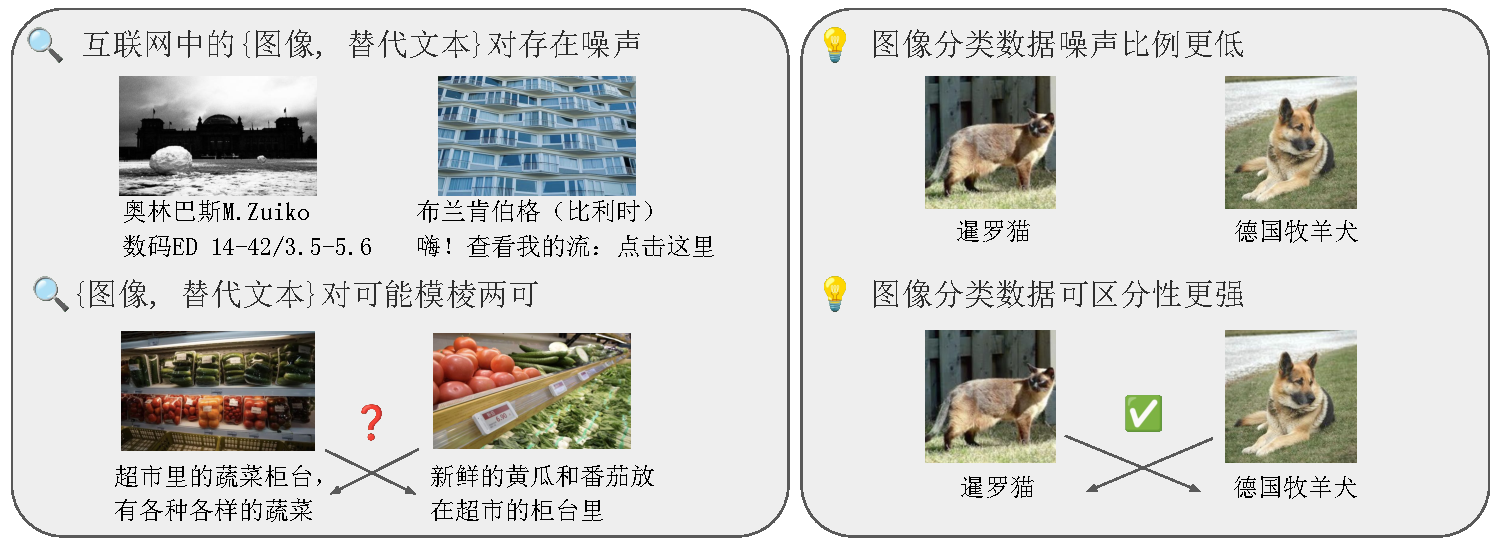
\includegraphics[width=1.0\linewidth]{figures/论文-iCLIP-概要.pdf}
  \caption{互联网图文对数据与图像分类数据的对比}
  \label{fig:iclip-overall}
\end{figure}

% 拜读了zl大哥DNL的部分,没想到引言部分是直接翻译过来的
\section{引言}
本章提出将对比学习思想扩展到其他图像及其标注信息配对数据中,从而合理利用已有的人工标注数据作为互联网图文对数据的补充,以实现不同标注形式的预训练数据的有效融合。
这种方式一方面为语言-图像对比学习方法提供额外的训练信号和图像样本,另一方面可以使用这些经过人工校对的精确标注信号作为视觉表征的准确锚定,增强其判别效果,使视觉表征与语言表征的联系更加紧密。
本章主要考虑有监督图像分类任务及其对应数据集作为语言-图像对比学习方法使用的图文对数据集的补充。
图像分类任务是一个典型的视觉预训练任务,其训练目标是在给定一组固定的预定义类别集合的情况下,将每一张输入图像划归到对应的类别。
作为有监督视觉预训练方法中最常使用的任务,研究界积累了相当多的公开图像数据。
如图\ref{fig:iclip-overall}右侧所示,广泛使用的ImageNet数据集\cite{deng2009imagenet}仔细标注了1400余万张图像,并将它们分为21841个不同的类别。其中每个类别都通过WordNet\cite{miller1995wordnet}语义网络提供了一个清晰的分类标准。因此图像分类任务的标注质量更高,同时具有明确的语义含义,更不容易出现不同的图像与标注之间混淆的情况,非常适合作为互联网图文对数据集的补充。
% 如果找到一种办法能有效利用这些现有的图像数据及其标注信息,并在实例级视觉-语言预训练方法中统一起来,将有效地提升整体数据的信噪比,并改善互联网图像文本对噪声导致的图文关联模糊问题。
% 同时,传统的图像分类任务往往仅限于一组预定义的固定类别集合,而CLIP方法天然具有开放类别的物体识别能力,这种表征融合的方法也很好地弥补了图像分类方法的不足。

% 本章将CLIP方法中的\{图像,文本\}实例级对比学习方法扩展到\{图像,文本,类别\}的三元组,在结合这两种视觉预训练方法的同时,充分利用对应的训练数据。
% 作为预实验,本章首先尝试了一个简单的多任务学习框架。该框架使用一个共享的视觉模型,并分别使用一个线性分类器进行图像分类任务训练和一个语言模型进行实例级多模态联合预训练。此时,\{图像,文本,类别\}的三元组关系通过分别建模\{图像,文本\}和\{图像,类别\}关系来实现。
% 虽然提升效果比较微弱,这种简单的多任务表征融合方法已经能够使两个单独的任务获益,但这一实验结果促进了本章沿着该方向的进一步探索。

因此本章探讨了如何有效地从语言-图像对比学习方法的角度重新理解传统的有监督图像分类方法。第一个尝试是将图像分类方法的损失函数和语言-图像对比学习方法的损失函数统一。
对比两者损失函数形式后可以发现,两种训练方法都可以被视作特殊的分类形式,其中前者是固定类别集合的分类,后者是正负样本对间的分类。
但两者仍然有几个主要区别:
1)损失函数形式不同。图像分类方法通常采用基于内积相似度的交叉熵损失函数,而语言-图像对比学习方法则使用基于余弦相似度的InfoNCE损失函数\cite{oord2018representation}。前者拟合能力更强,而后者对类别泛化更加友好。
% 1)损失函数形式不同。图像分类方法通常使用拟合能力较强的线性损失分类器。%由于线性损失的非归一化性质,该分类器驱动下的模型往往具有更好的拟合能力。
% 而语言-图像对比学习方法则采用对新类别泛化性更好的余弦损失分类器\cite{cao2020parametric,DengArcFace,wang2018cosface}。
2)分类器权重的参数化方法不同。图像分类方法采用直接类别参数化的分类器,而语言-图像对比学习方法则使用语言模型重参数化分类器。前者适合固定类别分类任务,后者适合多变类别分类任务。
% 图像分类方法只处理固定类别集合分类任务,可以直接优化各个类别的中心权重。而语言-图像对比学习方法则使用语言模型来建模不同文本中包含的语义信息,可以理解为通过语言模型重参数化了各个类别的中心权重。这种共享语义表征建模方式允许对不同文本语义之间的内部关系进行建模以增强对不同概念间关系的理解。同时这种方式可以处理预训练过程中未曾出现的概念信息,实现开放集合图像识别任务。
因此本章提出修改图像分类损失函数方法,从而与语言-图像对比学习方法统一。

除了统一损失函数形式之外,本章的第二个尝试是借助外部专家知识库增强数据,弥补图像分类数据和图文对数据在标注信息语义丰富度上的差异。
图像分类数据中提供语义信息的类别标签为求简洁明确,通常以一个或几个单词来表示。
但不同的类别标签之间可能有概念上的重叠,这使得它们在指代特定概念时存在有歧义情况。而图文对数据中提供语义信息的替代文本则通常是一个包含丰富语义的完整句子。这种语义信息密度的差异影响了语言模型的学习效果。
本方法利用了字典、百科等外部知识库来为图像分类数据中的类别标签提供更丰富的语义信息,包括类别定义、形象描述、与其他概念的关联和区别等等。这个过程就像人类通过真实示例和字典中的解释来学习新单词或概念,同时建模了这些新概念与其他概念间的关系。
% 为这些类别名称提供了为模型训练提供了更多监督信号。
得益于在图像分类方法中引入语言模型重参数化分类器的设计,这种包含了复杂语义信息的外部知识可以通过语言模型来直接建模,从而更好地从语言-图像对比学习方法的角度重新理解图像分类方法。

% 图像分类任务中类别名称为力求简洁明确,通常以一个或几个单词来表示。但不同的类别名称之间可能有概念上的重叠,这使得类别名称在指代特定语义时存在有歧义或多义的情况。
% 例如,ImageNet数据集中有一类别为``夜晚的鸟''(``night bird''),这一类别名称就与数据集中出现的其他类别有概念上的重叠,包括数据集中出现的``猫头鹰''(``owl'')、``夜莺''(``nightingale'')等类别。此外,``nightingale''还与知名历史人物弗洛伦丝·南丁格尔(``Florence Nightingale'')有词汇上的重合。% https://storage.googleapis.com/bit_models/imagenet21k_wordnet_lemmas.txt
% 与此同时,CLIP联合预训练方法使用图文对数据训练,其中的替代文本往往是包含丰富语义的完整句子。
% 为了进一步弥合图像分类任务和实例级视觉-语言多模态联合预训练任务之间的差距,
整合这些技术后,本章提出了一个新的预训练方法,称为iCLIP。iCLIP方法从损失函数和标注信息语义丰富度两个角度出发,以语言-图像对比学习方法重新理解传统的有监督图像分类方法,从而在基于互联网图文对数据的语言-图像对比学习预训练中得以有效融合高质量的图像分类数据,降低了数据噪声影响的同时增加了预训练可利用数据来源。

实验结果首先表明,尽管线性损失分类器和分类器权重直接参数化方法是图像分类方法的默认形式,但是将语言-图像对比学习方法的余弦损失分类器和语言模型重参数化分类器引入图像分类方法不会影响图像分类任务本身的学习效果。这一结果支持iCLIP方法用语言-图像对比学习思想有效融合两种方法的数据源进行预训练。
此外,iCLIP方法提出的外部专家知识库增强方法有效缩小了图像分类数据和图文对数据在标注信息的语义丰富度上的差距。实验表明将外部知识作为文本前缀或后缀与类别标签组合,即可显著提高模型的零样本开放集合图像识别任务效果,并改进了模型在零样本图文跨模态检索任务上的表现。
相比于简单的多任务预训练方法,这种从损失函数和标注信息语义丰富度角度重新理解图像分类方法,有效融合两种预训练方式的iCLIP方法显著提升了视觉表征与语言表征的对齐效果,并增强了视觉表征的语义判别能力。
与此同时,在迁移到下游视觉任务中时,iCLIP方法表现也更佳。相比于单一图像分类方法或单一语言-图像对比学习方法,iCLIP方法在少样本图像识别\cite{imagnettransfer}、ADE20K数据集\cite{zhou2019ade}语义分割、LVIS数据集\cite{gupta2019lvis}长尾类别物体检测和Kinetics-400数据集\cite{kay2017kinetics}视频动作识别等任务上均展现出优势。
% 这表明以实例级视觉-语言多模态联合预训练CLIP方法的形式重新理解和建模图像分类任务没有额外损失,因此可以

% 本章在不同规模的数据集组合实验中对该方法进行了验证。结果表明更高精度的图像分类数据明显增强了CLIP预训练对效果,使其在零样本物体识别和图文跨模态检索任务中的表现明显优于单独使用其中一种预训练方法或简单的多任务学习方法。

综上所述,本章的主要内容安排如下:
\begin{itemize}
    \item 第\ref{sec:iclip-intro}节讨论了互联网图文对数据中的标注噪声问题和引入高质量有标注数据,比如图像分类数据的潜在好处并介绍了从损失函数形式和标注信息语义丰富度两个角度,重新以语言-图像对比学习思想理解图像分类任务的方法。
    \item 第\ref{sec:iclip-method}节介绍了本章的研究方法,包括从对比学习角度理解图像分类任务的具体设计以及引入外部专家知识库对类别语义进行增强的具体方法等,并提出统一预训练方法iCLIP的具体实现。
    \item 第\ref{sec:iclip-result}节介绍了本章的实验设置、评测指标和实验结果,以及针对各模块的消融实验结果。
    \item 第\ref{sec:iclip-summary}节对本章内容进行了总结。
\end{itemize}

\section{研究方法}
在第\ref{sec:iclip-compare}节中首先对比了图像分类方法和语言-图像对比学习方法的损失函数。之后,在第\ref{sec:iclip-adapt-classification}节中提出从对比学习角度理解图像分类方法的具体设计,并在第\ref{sec:iclip-adapt-external}节中讨论了引入外部专家知识库对图像类别语义进行增强的做法。最后在第\ref{sec:iclip-unify}节中介绍了有效融合的统一预训练方法iCLIP的具体形式。

\label{sec:iclip-method}
\begin{figure}
  \centering
  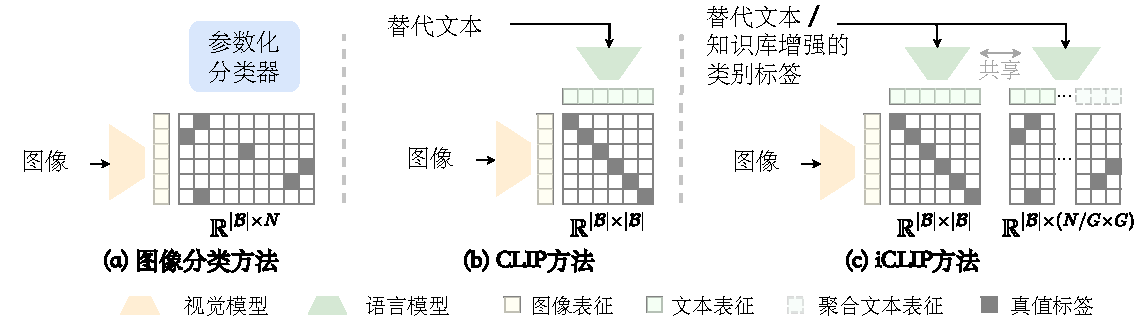
\includegraphics[width=1.0\linewidth]{figures/iclip-compare.pdf}
  \caption{图像分类方法、CLIP方法和融合后的iCLIP方法示意图}
  \label{fig:iclip-compare}
\end{figure}
\subsection{图像分类方法和语言-图像对比学习方法对比}
\label{sec:iclip-compare}
\paragraph{图像分类方法的损失函数} 图像分类方法的训练数据$D^{c}$是一组\{图像,类别序号\}对,记为$D^{c}={(I_{i}, C_{i})}_{i=1}^{|D^{c}|}$,其中$I_{i}$和$C_{i}$分别表示第$i$个图像和对应的类别序号标注。图像分类方法的训练目标是使用视觉模型$\theta_{I}$和直接参数化的类别分类器$h_{c}$预测给定图像的类别序号。分类器$h_{c}$是一个$N×H$大小的线性层,其中$N$是分类数据中的总类别数,$H$是视觉模型$\theta_{I}$输出的图像表征维度。分类器的参数记为$W$。图\ref{fig:iclip-compare}(a)展示了批大小为$\mathcal{B}$时的情况。
视觉模型$\theta_{I}$将每个图像$I_{i}$转换为图像表征:$v_{i}=\theta_{I}(I_{i})$,而分类器$h_{c}$则通过计算$W$和$v_{i}$之间的内积来预测该图像在所有类别上的概率分布$P_{i}$,且$P_{i}\in R^{N}$。最后,图像分类方法在$P_{i}$和$C_{i}$之间应用交叉熵函数来计算训练损失,公式化为:
\begin{equation}
 \mathcal{L}=-\frac{1}{\left|\mathcal{D}^{c}\right|} \sum_{\left(I_{i}, C_{i}\right) \in \mathcal{D}^{c}} \log \frac{\exp \left(W_{C_{i}} \cdot v_{i}\right)}{\sum_{j=1}^{N} \exp \left(W_{j} \cdot v_{i}\right)},
 \label{eq:iclip-classification}
\end{equation}
其中$W_{j}$是分类器参数中第$j$个类别对应的中心权重。

\paragraph{语言-图像对比学习方法的损失函数} 语言-图像对比学习方法的训练数据$D^{a}$是一组\{图像,替代文本\}对,记为$D^{a}={(I_{i}, T_{i}^{a})}_{i=1}^{|D^{a}|}$,其中$I_{i}$和$T^{a}_{i}$分别表示第$i$个图像和对应的文本标注。
语言-图像对比学习方法的训练思想是通过视觉模型$\theta_{I}$和语言模型$\theta_{T}$缩小配对的图像表征和文本表征之间的距离,同时扩大未配对的图像表征和文本表征之间的距离。
图\ref{fig:iclip-compare}(b)展示了批大小为$\mathcal{B}$时的情况。
语言-图像对比学习方法首先将图像$I_{i}$和替代文本$T_{i}^{a}$通过视觉模型$\theta_{I}$和语言模型$\theta_{T}$转换为对应表征$v_{i}$和$s_{i}$,也即$v_{i}=\theta_{I}(I_{i})$且$s_{i}=\theta_{T}(T_{i}^{a})$。接着,语言-图像对比学习方法应用InfoNCE对比损失函数来计算训练损失。以当前图像$I_{i}$为中心的损失函数公式化为:
\begin{equation}
 % \mathcal{L}=-\frac{1}{\left|\mathcal{D}^{a}\right|} \sum_{\substack{\left(I_{i}, T_{i}^{a}\right) \\ \in \mathcal{D}^{a}}} log \frac{exp \left(cos \left(\theta_{T}\left(T_{i}^{a}\right), v_{i}\right) / \tau\right)}{\sum_{T_{j}^{a} \in \mathcal{T}^{a}} exp \left(cos \left(\theta_{T}\left(T_{j}^{a}\right), v_{i}\right) / \tau\right)}
 \mathcal{L}=-\frac{1}{\left|\mathcal{D}^{a}\right|} \sum_{\left(I_{i}, T_{i}^{a}\right) \in \mathcal{D}^{a}} \log \frac{\exp \left(\cos \left(s_{i}, v_{i}\right) / \tau\right)}{\sum_{T_{j}^{a} \in \mathcal{T}^{a}} \exp \left(\cos \left(s_{j}, v_{i}\right) / \tau\right)},
 \label{eq:iclip-clip}
\end{equation}
其中$\cos(\cdot, \cdot)$表示两个表征之间的余弦相似度,$\mathcal{T}^{a}$是当前批数据中的所有文本标注作为对比对象,包括一个和当前图像$I_{i}$配对的正样本和$\mathcal{B}-1$个不配对的负样本,而$\tau$是一个缩放相似程度的超参数。由于语言-图像对比学习方法对图像信息和文本信息的建模对称性,在训练过程中还有一个以当前替代文本$T_{i}^{a}$为中心的损失函数,并取两者平均。该损失函数和公式\eqref{eq:iclip-clip}形式相似,只是将对比对象从当前批数据中的所有文本标注替换为所有图像。
 
\paragraph{损失函数对比} 比较图像分类任务和语言-图像对比学习方法的损失函数,可以看出两种训练方法都可以被视作分类方法的一种,前者在固定大小的图像类别中进行分类,后者则在给定批数据中的所有文本标注中进行分类。但是它们之间仍有三个主要区别:
\begin{itemize}
    \item 两种方法在损失函数形式上有区别。图像分类方法使用基于内积相似度的线性损失函数。由于内积相似度是一种非归一化的相似度,可以通过表征和参数的模长提供更多信息,该损失函数下的分类器往往具有更好的拟合能力。而语言-图像对比学习方法则采用基于余弦相似度的损失分类器。这种损失函数下的分类器更关注方向信息,对新类别泛化性更好\cite{cao2020parametric,DengArcFace,wang2018cosface}。
    % 1)损失函数形式的区别。图像分类任务通常采用基于内积相似度的交叉熵损失,而语言-图像对比学习方法则使用基于余弦相似度的InfoNCE损失函数\cite{oord2018representation}。
    \item 两种方法在分类器权重的参数化方法上有区别。图像分类方法采用直接参数化的类别分类器,这种分类器可以直接优化各个类别的中心权重,但只处理固定类别集合的分类任务。而语言-图像对比学习方法则使用一个语言模型来建模不同文本标注中包含的语义信息,可以理解为通过语言模型重参数化分类器权重。这种类别间共享参数的方式允许分类器构建不同类别间的复杂关系,增强对不同语义概念的理解。同时这种方式借助语言模型的灵活性,可以建模训练过程中未曾出现过的概念信息,从而实现开放集合图像识别的目标。
    % 图像分类方法采用直接参数化的类别分类器,而语言-图像对比学习方法则使用语言模型重参数化分类器。
    \item 两种方法在标注信息的语义丰富度上有区别。图像分类方法使用的类别序号仅仅区分了不同类别,并不包含任何语义信息,而语言-图像对比学习方法使用的文本标注是包含丰富语义的完整语句,提供了关于图像内容的详细描述。
\end{itemize}


\subsection{从对比学习角度重新理解图像分类方法}
\label{sec:iclip-adapt-classification}
为了有效融合图像分类任务和语言-图像对比学习方法,从而运用高质量图像分类数据进行增强,本节讨论了从对比学习角度重新理解图像分类方法的两个调整措施:对齐损失函数形式和统一分类器参数化方法。整体流程如图\ref{fig:iclip-adapt}所示。
% todo: 现在的写法里,a.2 & a.3要画成对齐损失函数和分类器参数化方法。

\begin{figure}
  \centering
  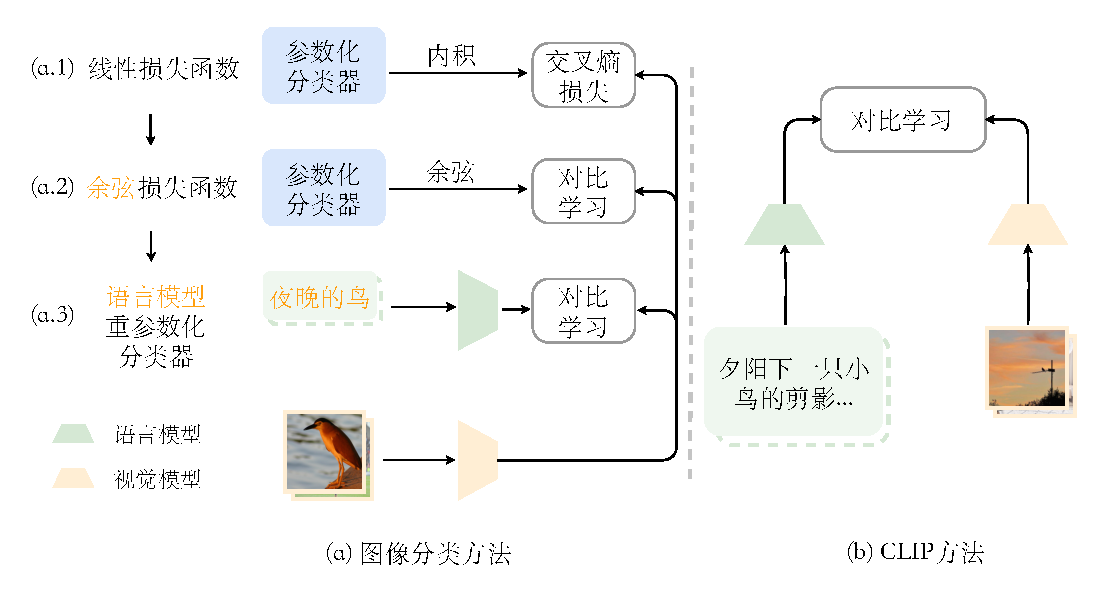
\includegraphics[width=1.0\linewidth]{figures/iclip-adapt-v2.pdf}
  \caption{从对比学习角度重新理解图像分类方法的调整措施}
  \label{fig:iclip-adapt}
\end{figure}

\paragraph{基于余弦相似度的图像分类损失函数} 如公式\eqref{eq:iclip-classification}所示,图像分类方法首先得到视觉表征$v_{i}$与直接参数化的类别分类器$h_{c}$之间的内积相似度,并归一化为概率分布$P_i$之后,与独热化类别序号之间应用交叉熵损失函数。这个损失函数与语言-图像对比学习方法中使用的InfoNCE对比损失函数相似但不一致,使得两个方法无法有效融合。
为了解决这个差异,本节提出在图像分类方法中引入余弦相似度,并同样添加一个控制概率分布的温度系数$\tau$,其损失函数形式就与InfoNCE对比损失函数形式一致,只是采样的负样本变成了其他类别。基于余弦相似度的图像分类损失函数公式化为:
\begin{equation}
    \mathcal{L}=-\frac{1}{\left|\mathcal{D}^{c}\right|} \sum_{\left(I_{i}, C_{i}\right) \in \mathcal{D}^{c}} \log \frac{\exp \left(\cos \left(W_{C_{i}}, v_{i}\right) / \tau\right)}{\sum_{j=1}^{N} \exp \left(\cos \left(W_{j}, v_{i}\right) / \tau\right)}.
    \label{eq:iclip-cosine}
\end{equation}

余弦相似度是度量学习\cite{nguyen2010cosine}中的一种常见做法。通过在图像分类方法中引入余弦相似度,图像分类方法与语言-图像对比学习方法在损失函数形式方面保持一致。后续实验表明,这种基于余弦相似度的图像分类方法可以取得与传统基于线性相似度的图像分类方法相当的分类表现。

\paragraph{在图像分类方法中引入语言模型重参数化分类器权重} 虽然公式\eqref{eq:iclip-cosine}对齐了两种方法的损失函数形式,但是两种方法使用的图像标注信息,也即图像分类数据中的类别序号和图文对数据中的文本内容,仍分别由直接参数化的类别分类器$h_{c}$和语言模型$\theta_{T}$进行建模。
在这种方式下,视觉模型接收到的训练信号由两个分类器单独给出,而且不同的语义概念信息无法在两个分类器间共享,无法充分利用文本语义概念丰富性和类别信息准确性的结合优势。
% 语言模型的学习信号并没有获得引入图像分类数据后的收益。
后续实验也表明,这种简单融合的分类器分离方案没有充分利用图像分类数据和图文对数据的优势,影响了预训练模型视觉表征与语言表征的对齐效果。

为了解决这个问题,本节重新引入图像类别中蕴含的语义信息,并提出用语言模型重参数化分类器建模图像分类任务。
如前文所述,图像分类数据集ImageNet中的每一个类别序号都对应了语义网络WordNet中的一个同义词集合,因此图像分类任务中的类别序号都有其对应的标签文本。因此,本节提出用共享的语言模型$\theta_{T}$重参数化图像分类方法的分类器权重。
具体而言,先通过语义网络WordNet将类别序号$C_{i}$替换为其对应的标签文本$M_{i}$,并通过语言模型$\theta_{T}$提取$N$个不同类别对应的文本表征,从而动态生成分类器权重$W$。在图像分类方法中引入语言模型重参数化分类器权重后的公式为:
\begin{equation}
    \mathcal{L}=-\frac{1}{\left|\mathcal{D}^{c}\right|} \sum_{\left(I_{i}, M_{i}\right) \in \mathcal{D}^{c}} \log \frac{\exp \left(\cos \left(\theta_{T}\left(M_{i}\right), v_{i}\right) / \tau\right)}{\sum_{j=1}^{N} \exp \left(\cos \left(\theta_{T}\left(M_{j}\right), v_{i}\right) / \tau\right)}.
    \label{eq:iclip-wo-dictionary}
\end{equation}

此时,语言模型$\theta_{T}$不仅有效捕获高区分度的标签文本语义特征,还能整合丰富的文本语义信息。
这一改进使得语言-图像对比学习方法可以更好地利用图像分类数据进行增强。

\subsection{外部专家知识库增强图像类别语义方法} 
\label{sec:iclip-adapt-external}
\begin{figure}
  \centering
  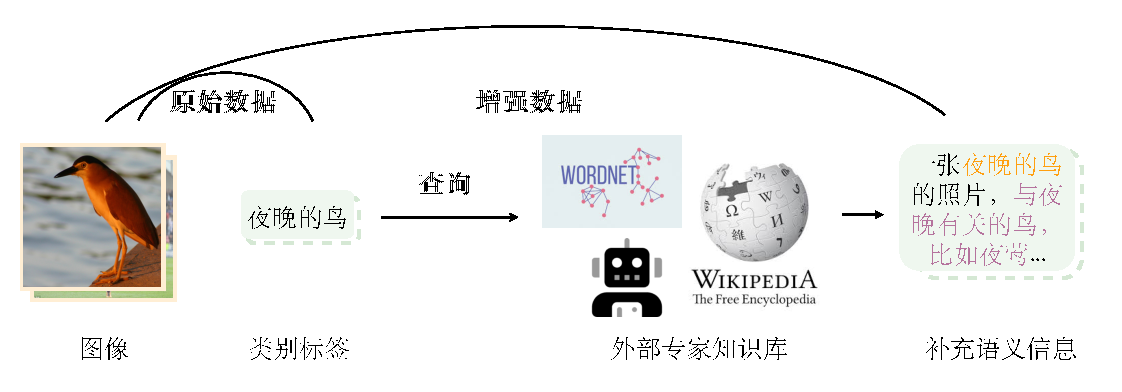
\includegraphics[width=1.0\linewidth]{figures/iclip-knowledge.pdf}
  \caption{外部专家知识库对类别标签的增强方法}
  \label{fig:iclip-knowledge}
\end{figure}
第\ref{sec:iclip-adapt-classification}节中通过引入基于余弦相似度的图像分类损失函数和语言模型重参数化分类器权重的方式,实现了从对比学习角度重新理解图像分类方法,并在很大程度上统一了两个不同的方法。
但是两种方法使用的数据在标注信息的语义丰富度上仍有较大区别。图像分类方法中类别对应的标签文本$M_i$来自于语义网络中的同义词集合。为保持简洁明确,通常每个类别均以一个或几个单词来表示。与此同时,语言-图像对比学习方法使用的图文对数据中,每个图像对应的文本标注包含了丰富的语义信息,其通常以完整语句的形式描述了图像中存在的物体对象、物体属性、对象间关系、上下文背景信息等等。
因此,需要进一步在标注信息的语义丰富度上进行对齐,减少两种方法之间的差异,增强预训练模型的学习效果。

为了增强图像分类数据中的标注信息的语义丰富度,本节提出引入外部专家知识库进行增强的方法。流程如图\ref{fig:iclip-knowledge}所示。具体而言,对于分类数据中的每一个类别,该方法都从外部专家知识库中检索并构造相关的知识信息作为标签文本的补充。这个知识库可以是字典、百科、知识图谱或者大语言模型。
在实际实现中,本节利用了语义网络WordNet作为外部专家知识库。如前文所述,每个分类类别在语义网络中都对应了一个同义词集合,而语义网络类似字典,为每个同义词集合编写了一条详细描述,用以明确定义该同义词集合所表达的语义概念,并可能提供一些相关知识以及与其他同义词之间的关联关系作为补充,非常适合作为外部知识引入。
得到每个类别对应的详细描述之后,该方法将其与类别标签文本组合并添加一些语法模板,使得新句子更加流畅易读,即可构成语义丰富度增强后的类别标注。这种增强后的标注称为图像类别描述,记作$\mathcal{T}^{c}$。
以“银行”类别为例,语义扩充后的类别标注为:“这是一张银行的图片,关于银行的定义是接受存款并将资金用于贷款活动的金融机构”。
% https://web.stanford.edu/~jurafsky/slp3/G.pdf

% 此外,在增强后的句子中。知识库增强后的类别标签形式为:
% \begin{equation}
%     \mathcal{T}^{c}=\{\text{TEMPLATE}\}_{C_i},\{\text{NAME}\}_{C_{i}},\{\text{DESCRIPTION} \}_{C_{i}}
%     \label{eq:iclip-format-label}
% \end{equation}

 这种外部专家知识库增强后的类别描述具有与图文对数据的文本信息相似的语义丰富度,从而进一步对齐了图像分类方法与语言-图像对比学习方法,以充分利用两种数据源。
 此外,这些外部专家知识库为每个图像类别引入了更多细节信息,能够减少因为原始的类别标签文本之间概念重叠造成的混淆现象。由于图像类别的标签文本本身长度较短,在类别数目较多的情况下容易存在指代特定语义时出现歧义的现象。
 例如,图像分类数据集ImageNet中有一类别为“夜晚的鸟”(“night bird”),这一类别名称就与数据集中出现的其他类别有概念上的重叠,包括“猫头鹰”(“owl”)和“夜莺”(“nightingale”)等类别。此外,“夜莺”的英文名称还与知名历史人物弗洛伦斯·南丁格尔护士(“Florence Nightingale”)有词汇上的相似。
 因此,仅仅依靠图像类别的标签文本难以区分不同类别间的细微差别,会影响模型在预训练过程中学习到更精确的概念表示。
 但是语义网络中将“夜晚的鸟”详细描述为“任何与夜相关的鸟类:猫头鹰、夜莺、夜鹰......”,提供了关于该类别更明确的语义信息。因此引入外部专家知识库的方法不仅在标注信息语义丰富度上与图文对数据对齐,还有助于模型区分不同概念并建立相关关系,进一步增强视觉表征的判别能力。

% 图像分类任务中类别名称为力求简洁明确,通常以一个或几个单词来表示。但不同的类别名称之间可能有概念上的重叠,这使得类别名称在指代特定语义时存在有歧义或多义的情况。
% 例如,ImageNet数据集中有一类别为``夜晚的鸟''(``night bird''),这一类别名称就与数据集中出现的其他类别有概念上的重叠,包括数据集中出现的``猫头鹰''(``owl'')、``夜莺''(``nightingale'')等类别。此外,``nightingale''还与知名历史人物弗洛伦丝·南丁格尔(``Florence Nightingale'')有词汇上的重合。% https://storage.googleapis.com/bit_models/imagenet21k_wordnet_lemmas.txt
% 与此同时,CLIP联合预训练方法使用图文对数据训练,其中的替代文本往往是包含丰富语义的完整句子。
% 为了进一步弥合图像分类任务和实例级视觉-语言多模态联合预训练任务之间的差距,

\subsection{有效融合的统一预训练方法iCLIP}
\label{sec:iclip-unify}
通过从对比学习角度重新理解图像分类方法并引入外部专家知识库增强图像类别语义,图像分类任务在损失函数形式、分类器权重参数化方法和标注信息语义丰富度三个方面,与语言-图像对比学习方法对齐。因此,本节提出了一个有效融合的统一预训练方法iCLIP,达到增强视觉表征的语义丰富度的效果。
如图\ref{fig:iclip-compare}(c)所示,iCLIP方法将高质量图像分类数据引入语言-图像对比学习预训练中,并用对比学习方法统一建模,其形式为:
\begin{equation}
   \mathcal{L}=-\frac{1}{|\mathcal{D}|} \sum_{\left(I_{i}, T_{i}\right) \in \mathcal{D}} \log \frac{\exp \left(\cos \left(\theta_{T}\left(T_{i}\right), v_{i}\right) / \tau\right)}{\sum_{T_{j} \in \mathcal{T}} \exp \left(\cos \left(\theta_{T}\left(T_{j}\right), v_{i}\right) / \tau\right)},
   \label{eq:iclip-unified}
\end{equation}
其中$D$是由图像分类数据集$D^{c}$和图文对数据集$D^{a}$组成的集合。而对比样本集合$\mathcal{T}$表示所有类别经过外部知识库增强后的标签文本集合$\mathcal{T}^{c}$或者当前批数据中的替代文本集合$\mathcal{T}^{a}$。因此,其中的文本信息$T_{j}$可以是从$\mathcal{T}^{c}$中采样的图像类别描述,或者从$\mathcal{T}^{a}$中采样的替代文本。
值得注意的是,在这个融合后的预训练方法中,视觉模型$\theta_{I}$和语言模型$\theta_{T}$在图像分类数据集和图文对数据集之间共享。这种融合方式使得模型能够借助图像分类数据集学习判别性更强的视觉表征,同时从图文对数据集中对齐更丰富的语义概念,增强了预训练效果。

\paragraph{通过分布式计算进行实现上的优化} 在iCLIP方法中,每个图像类别描述对应的语言表征由同一个语言模型动态生成,以替代直接优化分类器权重$W$的传统做法。当图像分类数据集中的类别数量$N$较小时,计算开销较小。
但是,对于图像类别数量$N$较大的数据集,例如包含2万多个类别的ImageNet数据集全集,在单次随机梯度下降过程中语言模型需要提取$N$个图像类别描述对应的语言表征,对训练速度产生了较大影响。
为了使iCLIP方法适用于尽可能多的图像类别,本节参考数据并行方法,实现了分布式训练策略\cite{chen2020simple}来降低由于图像类别增多造成的计算开销。
具体来说,iCLIP方法将$N$个引入外部专家知识库增强后的图像类别描述均匀地分布在$G$个数据并行的模型实例上,使得每个模型实例只需要提取$N/G$个图像类别描述对应的语言表征。在计算公式\eqref{eq:iclip-unified}的损失函数时,每个模型实例会从其他模型实例中的输出中收集对应类别的语言表征以构建完整集合,再与分配给当前模型实例的图像进行对比学习。
这种分布式计算方法显著降低了语言模型提取表征的计算成本,并节约了$(G-1)/G$的显存开销,使得iCLIP方法能够处理图像类别数量较大的分类数据集。

\section{实验结果}
\label{sec:iclip-result}
本节将有效融合的统一预训练方法iCLIP,与单方法预训练基线和简单融合预训练基线进行比较。实验验证了引入高质量图像分类数据后对语言-图像对比学习方法的增强效果。
本节分别在百万、千万和亿级别数据规模上对iCLIP方法进行了验证,验证所提方法在不同的数据规模下均能表现出更优性能,并在小规模数据集上进行详细的消融实验。
为比较增强前后语言-图像对比学习方法预训练效果,本节采用零样本开放集合图像识别任务和零样本图文跨模态检索任务对各个方法进行比较,反映了不同方法的视觉表征与语言表征对齐水平和视觉表征对语义概念的覆盖程度。与此同时,本节还在各类视觉下游任务上验证不同预训练方法的微调效果,包括图像语义分割任务、长尾类别物体检测任务和视频动作识别任务。

\subsection{实验设置}
\label{sec:iclip-exp-setting}
本节首先详细说明预训练过程中使用的数据集和实验设置,以及评测方法。

\paragraph{预训练实验数据和设置} 本节使用百万、千万和亿级别三种不同规模的数据集组合进行预训练实验,以充分比较不同方法在不同规模下的表现。
\begin{itemize}
    \item 在百万级图像规模的实验设置中,本节选用常用的ImageNet 1K子集(简称为IN-1K)和Conceptual Caption 3M数据集\cite{sharma-etal-2018-conceptual}(简称为CC-3M)作为预训练数据。作为图像分类数据,IN-1K数据集大约有128万张图片,并包含1000种不同的图像类别,而CC-3M数据集则是图文对数据集,大约有300万张图片,每张图片有一个配对的替代文本。
    在模型结构方面,视觉模型采用Swin-Tiny\cite{Swin}结构,约有2800万个参数,并使用224x224像素的图片作为输入,而语言模型则采用BERT-Base\cite{BERT}结构,约有1亿2500万个参数,并最多使用77个词元的文本作为输入。视觉模型和语言模型分别通过视觉自监督方法MoBY\cite{MoBY}和语言自监督方法RoBERTa\cite{liu2019roberta}进行初始化,从而加速实验收敛速度,节约预训练的计算开销。
    在每一个批大小为$\mathcal{B}$的训练批次中,iCLIP方法分别从两个数据集采样一半的图像,因此两个数据源的总训练样本数相同。所有实验中的单模型实例的批大小为128张图像,并使用分布式数据并行方法在8个模型实例上并行训练了100轮。默认的学习率调度为余弦调度方法,其中前5轮会进行学习率预热至2e-4的最高学习率。在正则化方面,实验的权重衰减系数为0.01,并使用随机增强\cite{cubuk2020randaugment}的图像数据增强方法和比例为0.1的随机深度\cite{huang2016deep}方法,以增强模型的泛化性。
    \item 在千万级图像规模的实验设置中,本节选用ImageNet全集(简称为IN-22K)和YFCC 14M子集\cite{YFCC100M}(简称为YFCC-14M)作为预训练数据。作为图像分类数据,IN-22K数据集大约有1400万张图片,并包含2万多种不同的图像类别,而YFCC-14M数据集是YFCC图文对数据集\cite{YFCC100M}的常用子集,同样包含大约1400万张图片。相比于前一组预训练数据设置,该组实验数据规模扩大了一个数量级,以进一步验证iCLIP方法的在更大规模数据上是否仍然有效。
    在模型结构方面,视觉模型同样使用Swin-Tiny结构,而语言模型则和原始CLIP语言模型\cite{radford2021learning}结构相同,使用一个隐藏宽度为512,深度为12层的Transformer\cite{Transformer}结构,约有6300万个参数。本组实验中的视觉和语言模型均从随机初始化开始训练,以便与一些相关工作进行公平的比较。
    在该组实验中采用的单模型实例批大小为512张图像,并在16个模型实例上并行训练了32轮。由于该组实验预训练长度增加,需要更强的正则化方法以防止过拟合,因此将权重衰减增大为0.05,而其他正则化设置和实验设置与之前相同。% 最大学习率设为2e-4或8e-4。
    此外,为与单方法预训练基线进行公平比较,本组实验设置了两个数据规模相当的变体:1)从IN-22K数据集中去除属于IN-1K数据集类别的所有数据,构造新的图像分类数据集IN-21K,用于评估IN-1K数据集上零样本图像识别效果;2)从IN-21K数据集和YFCC-14M数据集中各采样一半数据进行组合,确保数据规模和训练开销与基线方法相同。
    \item 在亿级别图像规模的实验设置中,本节选用ImageNet全集和Laion-400M数据集\cite{schuhmann2021laion400m}作为预训练数据。Laion-400M数据集是一个从Common Crawl开源项目中收集的超大规模图文对数据集,包含大约4亿张来源各异、内容丰富的图像,可以充分验证iCLIP方法在超大规模数据组合下是否仍然有效。
    在该组实验设置中,视觉模型采用Swin-Base\cite{Swin}结构,约有8900万参数,而语言模型仍使用BERT-Base结构,并采用自监督方法对模型进行初始化。
    整个实验共训练10万个批次,其中单模型实例的批大小为192张图像,并采用64个数据并行的模型实例同时预训练。和前述实验设置略有不同,本组实验在每个批大小为192的训练批次中,分别从IN-22K数据集和Laion-400M数据集中采样64张和128张图像。因此,本组实验在图像分类数据集上完成约30轮训练,在图文对数据集上完成约2轮训练。
    在实验设置方面,本组实验同样使用余弦学习率调度方法,并使用前16700个训练批次进行学习率预热至到1e-3的最高学习率。在正则化设置方面,模型的权重衰减系数设置为0.05,随机深度比例设置为0.2,其他设置不变。
\end{itemize}

\paragraph{评测数据集和微调设置} 本节通过两种评测方法比较不同预训练方式的视觉表征训练效果,并在几种不同的微调任务中对不同预训练方法进一步对比。
\begin{itemize}
    \item 零样本开放集合图像识别任务是语言-图像对比学习方法的重要评测方式之一。本节在三个评测集上对比了不同预训练方法视觉表征的语义丰富度和泛化能力:1)IN-1K评测集及其变体IN-S评测集\cite{wang2019learningSketch}上的Top-1准确率,衡量了通用图像识别能力和视觉表征的健壮性;2)广泛使用的Kornblith-12评测集\cite{imagnettransfer}上的平均Top-1准确率,涵盖了12个不同领域的开放集合细粒度图像识别任务;3)UniCL\cite{unicl}方法中使用的14个细粒度图像识别任务的平均Top-1准确率,简称为UniCL-14泛化评测集。
    \item 领域内的图像识别任务是一种特殊的图像识别任务评测。一些预训练设置中包含了IN-1K训练数据集,因此在这些情况下在IN-1K和IN-S评测集上测试反映了不同方法在领域内的图像识别能力,不涉及开放集合识别能力。
    \item 零样本图文跨模态检索任务评测衡量了语言-图像对比学习方法的视觉表征与语言表征对齐效果。本节使用包含1000张图片的Flickr30K\cite{young2014flickr}(简称Flickr)评测集和包含5000张图片的MSCOCO\cite{chen2015microsoft}(简称COCO)评测集上对不同预训练方式进行比较,并展示不同方法在这两个评测集上的图像检索(简称为IR)和文本检索(简称为TR)的Top-1召回率。
    \item 在下游视觉任务上的微调表现反映了不同预训练方法视觉模型的泛化能力。本节首先评价了不同方法在少样本图像识别任务上的微调表现。该任务使用Kornblith-12数据集上的训练集对模型进行微调,并根据每个图像类别的训练样本数目不同构造了不同的评测方式。这项微调任务设置遵循了OpenAI CLIP\cite{radford2021learning}工作的原本设置:在微调过程中固定视觉模型不变,只微调额外的类别分类器,并报告平均Top-1准确率。
    其次,本节还在图像语义分割、长尾类别物体检测和视频动作识别视觉任务上对不同预训练方法进行了微调,并分别比较了不同方法在这些任务上的mIoU得分、检测框mAP得分和Top-1准确率。具体的微调设置如下。针对图像语义分割任务,本节使用MaskFormer~\cite{maskformer}方法作为微调框架在ADE20K\cite{zhou2019ade}数据集进行实验,将其视觉模型的窗口大小设为7,其他设置与其默认训练超参数配置一致,并展示了单尺度测试结果。对于长尾类别物体检测任务,本节使用了包含1203个不均匀分布物体类别的LVIS数据集\cite{gupta2019lvis},并采用广泛使用的Faster R-CNN\cite{ren2016faster}方法作为微调框架。其他微调设置与主流方法\cite{Swin}一致,包括24轮的训练时长、图像短边长度在480-800像素之间的多尺度训练,并报告单尺度检测框的测试结果。对于视频动作识别任务,本节采用Swin视觉模型的微调框架和设置,在Kinetics-400\cite{kay2017kinetics}数据集上微调30轮,并报告Top-1准确率。
\end{itemize}

\subsection{百万级图像规模的组合实验}
\begin{table}
  \centering
  % \addtolength{\tabcolsep}{+1.0pt}
\caption{从对比学习角度重新理解图像分类方法的消融实验}
  \begin{tabular}{lcccc}
    \toprule
    序号 & 损失函数对齐 & 分类器对齐 & 标注语义对齐 & IN-1K Top-1准确率(\%) \\
    %\hline
    % \cmidrule(lr){1-1}\cmidrule(lr){2-4}
    % \cmidrule(lr){5-5}
    \midrule
    \#1 & & & & 80.9  \\
    \#2 & $\checkmark$ & & & \textbf{81.5} \\
    \#3 & $\checkmark$ & $\checkmark$ & & 81.2  \\
    \#4 & $\checkmark$ & $\checkmark$ & $\checkmark$ & 81.4 \\
    \bottomrule
  \end{tabular}
  \label{tab:iclip-ablate_head}
\end{table}

\paragraph{从对比学习角度重新理解图像分类方法的消融实验}
表\ref{tab:iclip-ablate_head}首先分析了重新理解传统图像分类方法对领域内图像识别能力的影响,因此该组实验只使用了IN-1K图像分类数据集,并报告IN-1K评测集上的Top-1准确率。第\ref{sec:iclip-adapt-classification}节和第\ref{sec:iclip-adapt-external}节中分别提出对齐图像分类损失函数方法、对齐分类器类型方法和对齐标注语义丰富程度方法。该组实验对这些方法进行了消融实验。% 本组实验使用IN-1K评测集Top-1的准确率反映图像分类任务本身的效果变化。
对比序号\#1与\#2的实验结果可以看出基于余弦相似度的图像分类损失函数在领域内图像识别任务上的性能略好于传统基于内积相似度的线性损失函数,因此在IN-1K评测集上有0.6\%的小幅提升。而进一步引入语言模型重参数化分类器权重方法和外部专家知识库增强图像类别语义方法后,图像分类任务本身的预训练效果基本保持不变。与原始图像分类方法相比,重新理解的图像分类方法在IN-1K评测集上仍有0.5\%的小幅增益。
这组实验结果表明从对比学习角度重新理解图像分类方法是可行的,为iCLIP方法通过语言-图像对比学习方法融合两类数据的策略提供有利支撑。

\begin{table}
  \centering
\caption{iCLIP方法与单预训练方法和简单融合方法的对比实验}
% 对于仅使用 IN-1K 的模型,我们训练它们 100 个 epoch。对于仅使用 GCC-3M 的模型,我们使用与 IN-1K 中使用的相同的迭代和批量大小来训练它们。
  \begin{tabular}{lcccc}
    \toprule
    \multicolumn{1}{c}{} &
    \multicolumn{1}{c}{} & 
    \multicolumn{1}{c}{Kornblith-12评测集}
    & \multicolumn{2}{c}{IN-1K和IN-S评测集} \\
    % \cmidrule(lr){1-1}\cmidrule(lr){2-2}
    % \cmidrule(lr){3-3}\cmidrule(lr){4-5}
    \midrule
    序号 & 方法 & 平均Top-1准确率(\%) & \multicolumn{2}{c}{Top-1准确率(\%)} \\
    %\hline
    % \cmidrule(lr){1-1}\cmidrule(lr){2-2}
    % \cmidrule(lr){3-3}\cmidrule(lr){4-5}
    \midrule
    \#1 & 仅图像分类方法 & - & \textbf{80.9} & 29.4 \\
    \#2 & 仅对比学习方法 & 31.4 & 32.4 & 18.3  \\
    % 3 & \emph{Split head (Sup.)} & - & 50.7 & 80.6 & 38.3 \\
    % 4 & \emph{Split head (Text)} & 35.1 & 54.9 & 45.0 & 24.7 \\
    \#3 & 简单融合基线 & 35.1 & 80.6 & 38.3 \\
    \#4 & iCLIP-NoD & 37.7 & 80.5 & 38.6 \\
    \#5 & iCLIP & \textbf{39.1} & 80.4 & \textbf{38.7} \\
    \bottomrule
  \end{tabular}
  \label{tab:iclip-ablate_cc}
\end{table}

\paragraph{在CC-3M图文对数据中引入IN-1K图像分类数据进行增强}
通过之前对图像分类方法的重新调整,本组实验进一步探究了iCLIP方法相比于单预训练方法和简单融合方法的性能提升。
其中简单融合基线是一种简单融合两种不同方法和训练数据集的预训练方法。该基线使用共享的视觉模型处理图像,但保留独立的直接参数化类别分类器和语言模型分别处理图像分类任务和语言-图像对比学习任务。因此这组基线只是将公式\eqref{eq:iclip-classification}与公式\eqref{eq:iclip-clip}两个损失函数直接平均以进行多任务预训练。
实验结果如表\ref{tab:iclip-ablate_cc}所示,与序号为\#1和\#2的单预训练方法基线相比,序号\#3对应的简单融合基线已经对模型零样本开放集合图像识别能力有了一定提升,并在Kornblith-12评测集上有3.7\%的平均Top-1准确率提升。此外,这种做法也保持了预训练模型在领域内的图像识别任务上的表现,并增强了视觉表征的健壮性。

为了进一步讨论外部专家知识库增强图像类别语义方法对预训练效果增强的效果,本组实验构造了在iCLIP方法中去除这一做法的基线,称之为iCLIP-无描述增强,简称为iCLIP-NoD。对比序号\#3对应的简单融合基线与序号\#4对应的iCLIP-NoD基线的实验结果,融合后的方法在Kornblith-12评测集上有2.6\%的准确率提升,且在IN-1K评测集及其变体上表现相当,说明引入语言模型重参数化分类器权重能有效融合两种预训练方法。
再将iiCLIP-NoD基线与序号为\#1和\#2的单预训练方法基线进行对比,有效融合后的模型在领域内的图像识别任务上的能力没有明显变化,在IN-1K评测集上比单图像分类方法基线低0.4\%。但在零样本开放集合图像识别任务上,相比于单语言-图像对比学习方法基线,在Kornblith-12评测集上有6.3\%的平均Top-1准确率提升,说明在语言-图像对比学习方法中引入高质量图像分类数据,可以显著增强语言-图像对比学习方法得到的视觉表征的语义覆盖度,提高对开放集合类别的识别能力。
% 同时将其与简单融合基线\#3相比,在 Kornblith-12数据集零样本物体识别任务上的平均Top-1准确率高出 2.6\%,而它们在IN-1K评测集及其变体上表现相当。这一结果说明iCLIP方法将图像分类任务重构并与实例级语言监督任务有效融合,能更好地汇聚两种学习方案的优点。
此外,引入外部专家知识库增强图像类别语义之后,序号\#5对应的iCLIP方法在Kornblith-12数据集上得到进一步改进,平均Top-1准确率提升了1.4\%。这进一步展示了对齐不同任务的标注信息语义丰富度后,模型在细粒度概念区分和图像识别能力上有所提升。


\subsection{千万级图像规模的组合实验}
本组实验将数据验证规模从之前的IN-1K与CC-3M数据组合扩展了一个数量级,以进一步验证iCLIP方法在更大规模和类别数更多的数据组合上的性能表现。

\paragraph{在YFCC-14M图文对数据中引入IN-22K图像分类数据进行增强} 与前述实验类似,本组实验也比较了引入高质量图像分类数据前后对语言-图像对比学习方法预训练效果的影响。在本组实验中,除了使用领域内和零样本开放集合图像识别任务对不同预训练方法进行评测,还评测了不同方法零样本图文跨模态检索的能力,展示了视觉表征与语言表征的对齐程度。
如第\ref{sec:iclip-exp-setting}节所述,本组实验中包括三种数据组合变体:1)组合一:IN-21K和YFCC-14M数据集各半,以评测iCLIP方法数据利用效率;2)组合二:完整IN-21K和YFCC-14M数据集组合,以评测IN-1K评测集上的零样本图像识别能力;3)组合三:IN-22K和YFCC-14M数据集组合,以评测IN-1K评测集上的领域内图像识别能力。

\begin{table}
    \centering
    \caption{引入图像分类数据增强语言-图像对比学习方法图像识别能力的实验}
    % 模型从头开始预训练的 32 个轮次。COCO 和 Flickr 代表 MSCOCO [31] 和 Flickr30K [64]。IR 和 TR 代表图像检索和文本检索。
    \begin{tabular}{lcccc}
    \toprule
        \multicolumn{1}{c}{} &
        \multicolumn{1}{c}{} & \multicolumn{1}{c}{} & \multicolumn{2}{c}{领域内和零样本开放集合图像识别任务} \\
        % \cmidrule(lr){1-1}
        % \cmidrule(lr){2-3}
        % \cmidrule(lr){4-5}
        \midrule
        序号 & 数据 & 方法 & IN-1K评测集(\%) & UniCL-14泛化评测集(\%)  \\
        % \cmidrule(lr){1-1}
        % \cmidrule(lr){2-3}
        % \cmidrule(lr){4-5}
        \midrule
        % ImageNet-1K &  Swin-Tiny \\
        \#1 & YFCC-14M & CLIP & 30.1 & 36.3 \\

        \#2 & 数据组合一 & iCLIP-NoD & 39.4 & 45.4 \\  
                
        \#3 & 数据组合一 & iCLIP & \textbf{45.9} & \textbf{49.9} \\    
        
        % \cmidrule(lr){1-1}
        % \cmidrule(lr){2-3}
        % \cmidrule(lr){4-5}
        \midrule
        
        \#4 & 数据组合二 & iCLIP-NoD & 41.1 & 49.4  \\  
                
        \#5 & 数据组合二 & iCLIP & \textbf{50.9} & \textbf{54.4} \\   
        
        % \cmidrule(lr){1-1}
        % \cmidrule(lr){2-3}
        % \cmidrule(lr){4-5}
        \midrule        
        
        \#6 & 数据组合三 & iCLIP-NoD & 76.2 & 51.6 \\
        
        \#7 & 数据组合三 & iCLIP & \textbf{76.3} & \textbf{55.5} \\

        \bottomrule
    \end{tabular}
    % since official codebase doesn't support training.
    % top-1 acc for zero-shot recognition; rank@1 for cross-modal retrieval
    \label{tab:iclip-ablate_yfcc}
\end{table}
% 中的\#2、\#4和\#6三组结果展示了三种不同的数据集组合设置下iCLIP预训练方法的评测结果。与实例级语言监督方法——CLIP基线(\#1)相比,在使用数据量完全公平的实验组\#2下,iCLIP在IN-1K评测集上的零样本识别能力有8.3\%的较大收益,在14个细粒度泛化评测数据集上进行零样本物体识别效果上也有9.1\%的平均Top-1准确率提升。
\begin{table}
    \centering
    \caption{引入图像分类数据增强语言-图像对比学习方法跨模态检索能力的实验}
    % 模型从头开始预训练的 32 个轮次。COCO 和 Flickr 代表 MSCOCO [31] 和 Flickr30K [64]。IR 和 TR 代表图像检索和文本检索。
    \begin{tabular}{lcccccc}
    \toprule
        \multicolumn{1}{c}{} &
        \multicolumn{1}{c}{} & \multicolumn{1}{c}{} & \multicolumn{4}{c}{零样本图文跨模态检索任务(\%)} \\
        % \cmidrule(lr){1-1}
        % \cmidrule(lr){2-3}
        % \cmidrule(lr){4-7}
        \midrule
        序号 & 数据 & 方法 & Flickr-IR & Flickr-TR & COCO-IR & COCO-TR    \\
        % \cmidrule(lr){1-1}
        % \cmidrule(lr){2-3}
        % \cmidrule(lr){4-7}
        \midrule
        % ImageNet-1K &  Swin-Tiny \\
        \#1 & YFCC-14M & CLIP  & 21.5 & 37.9 & 12.5 & 21.2  \\

        \#2 & 数据组合一 & iCLIP-NoD  & 27.6 & 39.1 & 13.0 & 20.4 \\  
                
        \#3 & 数据组合一 & iCLIP & \textbf{31.9} & \textbf{49.8} & \textbf{15.5} & \textbf{27.2} \\    
        
        % \cmidrule(lr){1-1}
        % \cmidrule(lr){2-3}
        % \cmidrule(lr){4-7}
        \midrule
        
        \#4 & 数据组合二 & iCLIP-NoD & 33.4 & 51.2 & 16.3 & 26.5  \\  
                
        \#5 & 数据组合二 & iCLIP & \textbf{37.1} & \textbf{55.7} & \textbf{18.5} & \textbf{30.7} \\   
        
        % \cmidrule(lr){1-1}
        % \cmidrule(lr){2-3}
        % \cmidrule(lr){4-7}
        \midrule
        
        \#6 & 数据组合三 & iCLIP-NoD & 33.2 & 48.2 & 14.4 & 23.8 \\
        
        \#7 & 数据组合三 & iCLIP & \textbf{36.2} & \textbf{55.3} & \textbf{18.0} & \textbf{29.7} \\

        \bottomrule
    \end{tabular}
    % since official codebase doesn't support training.
    % top-1 acc for zero-shot recognition; rank@1 for cross-modal retrieval
    \label{tab:iclip-ablate_yfcc_retrieval}
\end{table}
表\ref{tab:iclip-ablate_yfcc}展示了领域内和零样本开放集合图像识别任务的评测结果。与序号\#1对应的单语言-图像对比学习方法相比,数据规模相当的实验组\#2iCLIP-NoD方法通过引入图像分类数据进行增强,在IN-1K评测集上的零样本图像识别任务上取得了9.3\%的Top-1准确率的显著提升,在UniCL-14泛化评测集上的零样本图像识别任务也有9.1\%的平均Top-1准确率提升。

表\ref{tab:iclip-ablate_yfcc_retrieval}展示了零样本图文跨模态检索任务的评测结果。对比序号\#1对应的单语言-图像对比学习方法,序号\#2对应的iCLIP-NoD方法在相对简单的Flickr30K图文跨模态检索基准上有一定的性能提升,但在更复杂的COCO图文跨模态检索基准上表现相当。
这一结果表明引入高质量图像分类数据后,语言-图像对比学习方法的视觉表征与语言表征对齐效果得到了一定的提升。但是不对齐的标注信息语义丰富度影响了语言模型的学习效果,引入外部专家知识库对图像类别语义进行增强方法可以有效缓解这一问题。
% 得到的新实例级语言监督预训练方法在数据利用效率方面都有较大提升。此外,考虑使用更多数据的情况,实验\#4和\#6两组在各个任务上都有进一步的提升。

\paragraph{外部专家知识库增强图像类别语义的效果} 
表\ref{tab:iclip-ablate_cc}的实验表明,外部专家知识库增强方法可以提升模型的零样本开放集合图像识别能力。但是其使用的图像分类数据为IN-1K数据集,仅包含1000种不同的图像类别,且不同类别间的标签文本区分性较好。本组实验进一步讨论了外部专家知识库增强图像类别语义方法在更大规模尤其是图像类别更多的数据集上的作用。
通过对比表\ref{tab:iclip-ablate_yfcc}中三组实验(\#2与\#3、\#4与\#5、\#6与\#7)可以发现,在三种不同的数据集组合设置下使用外部专家知识库将类别标签文本扩展为图像类别描述后,模型在零样本开放集合图像识别任务上均有明显的性能提升。
具体而言,在各自使用一半IN-21K和YFCC-14M数据集的数据组合一设置上,外部专家知识的引入使得语言-图像对比学习方法在IN-1K评测集上的Top-1准确率提高了6.5\%,在UniCL-14泛化评测集上的平均Top-1准确率提高了4.5\%。
此外,表\ref{tab:iclip-ablate_yfcc_retrieval}的实验也表明外部专家知识能够对齐不同数据集的标注信息语义丰富度,显著提升了预训练方法在零样本图文跨模态检索任务上的表现。% 对比表\ref{tab:iclip-ablate_yfcc}的序号\#2与\#3,序号\#4与\#5和序号\#6与\#7的实验组可以发现,外部专家知识库增强图像类别语义方法增强了iCLIP方法在所有图文跨模态检索基准上的表现。
% 对于图像检索文本任务,该方法可以在 Flickr30K和MSCOCO评测集上分别提升10.7\%和6.8\%的Top-1召回率,在文本检索图像任务上也有2\%到4\%的提升。
% 和图文检索任务上取得一致改进。

\begin{table}
    \centering
    % \addtolength{\tabcolsep}{-1.0pt}
    \caption{不同图像分类数据和图文对数据混合比例的消融实验}
    \begin{tabular}{lccccc}
    \toprule
        % \multicolumn{1}{c}{} &
        % \multicolumn{1}{c}{} & \multicolumn{1}{c}{} & \multicolumn{1}{c}{} & \multicolumn{2}{c}{Zero-shot retrieval} \\
        % \cmidrule(lr){1-1}
        % \cmidrule(lr){2-3}
        % \cmidrule(lr){4-4}
        % \cmidrule(lr){5-6}
        序号 & 训练数据混合比例 & 方法 & IN-1K & COCO-IR & COCO-TR    \\
        % \cmidrule(lr){1-1}
        % \cmidrule(lr){2-3}
        % \cmidrule(lr){4-4}
        % \cmidrule(lr){5-6}
        \midrule
        % ImageNet-1K &  Swin-Tiny \\
        \#1 & ~100\% YFCC-14M + 0\% IN-21K ~& CLIP & 30.1 & 12.5 & 21.2  \\

        \#2 & {90\% YFCC-14M + 10\% IN-21K} & iCLIP & 40.9 & 13.9 & 25.5 \\ 

        \#3 & {75\% YFCC-14M + 25\% IN-21K} & iCLIP & 43.9 & 15.2 & \textbf{27.5} \\ 
        
        \#4 & 50\% YFCC-14M + 50\% IN-21K & iCLIP & \textbf{45.9} & \textbf{15.5} & 27.2 \\    
        
        \#5 & {25\% YFCC-14M + 75\% IN-21K} & iCLIP & 44.8 & 14.1 & 27.1 \\  

        \#6 & {10\% YFCC-14M + 90\% IN-21K} & iCLIP & 44.2 & 14.9 & 25.9 \\
        \bottomrule
    \end{tabular}
    % since official codebase doesn't support training.
    % top-1 acc for zero-shot recognition; rank@1 for cross-modal retrieval
    \label{tab:iclip-ablate_combine}
\end{table}

\paragraph{混合不同比例图像分类数据的消融实验} 如第\ref{sec:iclip-exp-setting}节所述,本组实验的图像分类数据和图文对数据混合比例为各50\%。
不同数据集的规模可能不同。为了验证iCLIP方法的推广性,表\ref{tab:iclip-ablate_combine}中探究了YFCC-14M图文对数据集与IN-21K图像分类数据集不同混合比例下得到的模型在图像识别和图文跨模态检索任务上的表现,其中序号\#4实验为默认数据比例设置。
从表\ref{tab:iclip-ablate_combine}中结果可以看出,在不同的混合比例下,引入高质量图像分类数据后的iCLIP方法相比于单语言-图像对比学习CLIP方法,在零样本开放集合图像识别任务和图文跨模态检索任务上都有较大提升。其中,仅引入10\%的图像分类数据就对语言-图像对比学习方法的预训练效果带来显著提升,而当两种数据混合比例为各50\%时达到最佳性能。
% 特别地考虑海量级的(图像,替代文本)数据和规模有限的(图像,类别)数据的组合,仅引入1/10的图像分类数据就有非常显著的收益(见实验\#2)。

\begin{figure}
  \centering
  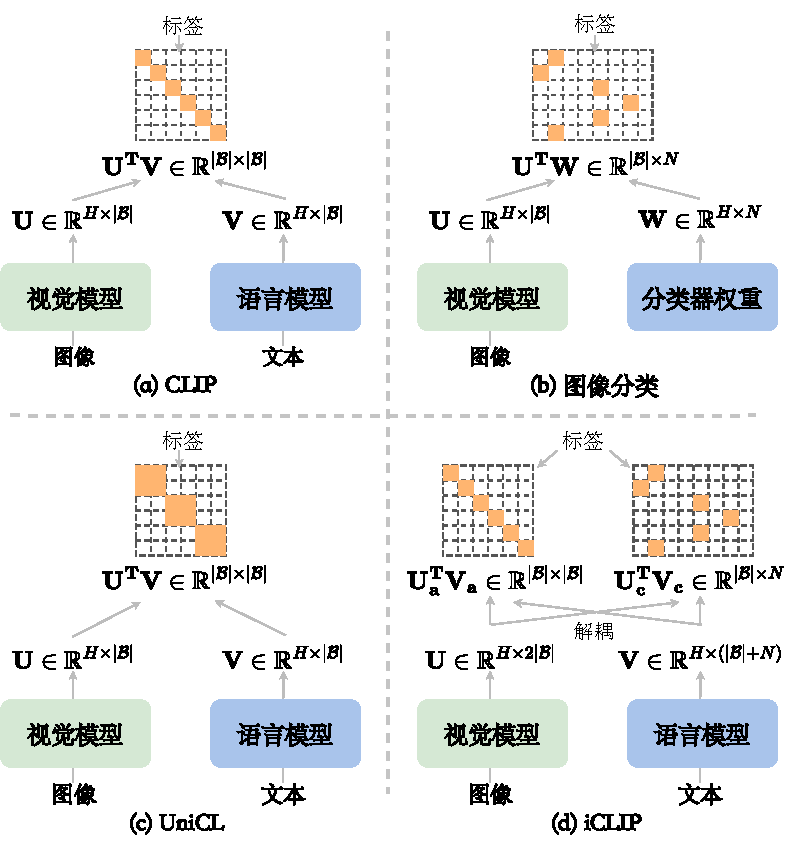
\includegraphics[width=0.8\linewidth]{figures/iclip-unicl.pdf}
  \caption{CLIP、图像分类、UniCL与本文iCLIP方法的对比图}
  \label{fig:iclip-unicl}
\end{figure}

\paragraph{与同期工作的比较} 
与本章工作同期也有一个工作UniCL\cite{unicl}采用了类似的想法:通过对比学习思想重新表达图像分类方法,从而与语言-图像对比学习方法进行有效融合,同样验证了本章介绍的基于高质量数据增强语言-图像对比学习预训练方法的有效性。
虽然两种方法具有相似的动机,但两者在方法设计上仍有两处较大区别,影响了方法融合程度和预训练效果。
% 对齐损失函数的基于余弦相似度的图像分类损失函数方法、对齐分类器类型的语言模型重参数化分类器权重方法、对齐标注语义丰富程度的外部专家知识库增强图像类别语义方法
首先,两种方法在如何融合两种预训练任务的设计上有区别。图\ref{fig:iclip-unicl}展示了CLIP方法、图像分类方法、UniCL方法与本节介绍的iCLIP方法的异同。
UniCL方法和iCLIP方法都在图像分类方法中引入了基于余弦相似度的损失函数和语言模型重参数化分类器权重方法,这使得两种数据集的标注信息,包括替代文本或图像类别,都可以通过共享的语言模型来建模,从而得以建立不同语义概念间的内部联系。

但两者在损失设计上并不相同。由于批大小的限制,同一批次内来自图像分类数据的图像只会覆盖全部$N$个图像类别中的一小部分。iCLIP方法会将这些图像与所有可能的类别名称进行对比学习,而UniCL方法只会将其与当前批次采样到的小部分类别名称进行对比学习,负样本对数量明显减小。
因此UniCL方法的损失设计很大程度上减小了图像分类数据可获取的训练信号,无法充分利用可区分性较高的图像分类标注信息。
% 此外,UniCL方法要求CLIP方法与图像分类的类别标签一起进行判别,由于替代文本语义涵盖更加丰富往往会涵盖类别名称,使得CLIP图文对的对比学习任务然而出现混淆情况。% 可能画个图可以说清楚
UniCL方法的损失设计优势在于无须设计并行训练架构。但如第\ref{sec:iclip-unify}节中所述,iCLIP方法提出了一个通过分布式计算的实现方案,可以将图像分类数据中涉及的所有类别均匀地分配给不同的并行模型实例,因此同样可以支持图像类别数较多的大规模图像分类数据的高效训练。%并在第\ref{sec:iclip-22k-laion}节中将其推广到亿级别的训练数据。

其次,两种方法的第二个主要区别在于iCLIP方法通过引入外部专家知识库,进一步缩小了图像类别的标签文本和图文对数据的替代文本间标注语义丰富度的差异。这种方法通过引入图像类别对应的额外语义信息,将类别标签文本扩展为内容更丰富的图像类别描述,提升了预训练视觉表征的语义丰富度,也提高了语言模型建模不同语义概念的能力。


\begin{table}
%\vspace{-0.5em}
    \centering
    % \addtolength{\tabcolsep}{-1.0pt}
    \caption{iCLIP方法与UniCL方法在图像识别能力上的对比实验}
    \begin{tabular}{lcccc}
    \toprule
        \multicolumn{1}{c}{} &
        \multicolumn{1}{c}{} & \multicolumn{1}{c}{} & \multicolumn{2}{c}{领域内和零样本开放集合图像识别任务} \\
        % \cmidrule(lr){1-1}
        % \cmidrule(lr){2-3}
        % \cmidrule(lr){4-5}
        \midrule
        序号 & 数据 & 方法 & IN-1K评测集(\%) & UniCL-14泛化评测集(\%)   \\
        % \cmidrule(lr){1-1}
        % \cmidrule(lr){2-3}
        % \cmidrule(lr){4-5}
        \midrule
        % ImageNet-1K &  Swin-Tiny \\
        \#1 & 数据组合一 & UniCL & 36.4 & 45.5 \\  
        \#2 & 数据组合一 & iCLIP & \textbf{45.9} & \textbf{49.9} \\  

        % \cmidrule(lr){1-1}
        % \cmidrule(lr){2-3}
        % \cmidrule(lr){4-5}
        \midrule
        
        \#3 & 数据组合二 & UniCL & 40.5 & 49.1 \\
        \#4 & 数据组合二 & iCLIP & \textbf{50.9} & \textbf{54.4} \\   

        % \cmidrule(lr){1-1}
        % \cmidrule(lr){2-3}
        % \cmidrule(lr){4-5}
        \midrule
        
        \#5 & 数据组合三 & UniCL & 70.5  & 52.4 \\
        \#6 & 数据组合三 & iCLIP & \textbf{76.3} & \textbf{55.5} \\

        \bottomrule
    \end{tabular}
    \label{tab:iclip-tounicl}
\end{table}

表\ref{tab:iclip-tounicl}展示了UniCL方法和iCLIP方法在IN-1K评测集和UniCL-14泛化评测集上的Top-1准确率,以对比两种方法在领域内和零样本开放集合图像识别任务上的表现。在三种不同的数据集组合设置下,iCLIP方法在IN-1K评测集上的Top-1准确率比UniCL方法至少高出5\%。具体而言,在数据组合三的实验中,由于预训练数据包含IN-1K图像类别,此时IN-1K评测集的结果反映了预训练方法的领域内图像识别能力。在该项任务上iCLIP方法仍明显优于UniCL方法,表明UniCL方法的损失设计并没有充分利用图像分类数据的训练信号。同时,在UniCL-14泛化评测集代表的零样本开放集合图像识别任务上,iCLIP方法也明显优于UniCL方法。实验结果表明,使用完整类别集合进行对比学习能够显著增强预训练视觉表征的判别能力。
% 同时在最大规模的IN-22K与YFCC-14M组合数据上,如实验序号\#6所示,iCLIP方法在泛化评测集上达到55.5\%的平均Top-1 准确率,比实验序号\#5的UniCL方法高3.1\%。
此外,表\ref{tab:iclip-tounicl-ret}中比较了UniCL方法和iCLIP方法在零样本图文跨模态检索任务上的性能,并展示了Flickr30K数据集和MSCOCO数据集上图像检索与文本检索任务的Top-1召回率。得益于第\ref{sec:iclip-adapt-external}节中提出的外部专家知识库增强图像类别语义做法,iCLIP方法在各个图文跨模态检索测试中均取得优于UniCL方法的表现。



\begin{table}
%\vspace{-0.5em}
    \centering
    % \addtolength{\tabcolsep}{-1.0pt}
    \caption{iCLIP方法与UniCL方法在图文跨模态检索能力上的对比实验}
    \begin{tabular}{lcccccc}
    \toprule
        \multicolumn{1}{c}{} &
        \multicolumn{1}{c}{} & \multicolumn{1}{c}{} & \multicolumn{4}{c}{零样本图文跨模态检索任务(\%)} \\
        % \cmidrule(lr){1-1}
        % \cmidrule(lr){2-3}
        % \cmidrule(lr){4-7}
        \midrule
        序号 & 数据 & 方法 & Flickr-IR & Flickr-TR & COCO-IR & COCO-TR    \\
        % \cmidrule(lr){1-1}
        % \cmidrule(lr){2-3}
        % \cmidrule(lr){4-7}
        \midrule
        % ImageNet-1K &  Swin-Tiny \\
        \#1 & 数据组合一 & UniCL & 21.5 & 37.9 & 12.5 & 21.2 \\  
        \#2 & 数据组合一 & iCLIP & \textbf{31.9} & \textbf{49.8} & \textbf{15.5} & \textbf{27.2} \\  

        % \cmidrule(lr){1-1}
        % \cmidrule(lr){2-3}
        % \cmidrule(lr){4-7}
        \midrule
        
        \#3 & 数据组合二 & UniCL & 34.0 & 50.3 & 17.7 & 28.0 \\
        \#4 & 数据组合二 & iCLIP & \textbf{37.1} & \textbf{55.7} & \textbf{18.5} & \textbf{30.7}\\   
        % \cmidrule(lr){1-1}
        % \cmidrule(lr){2-3}
        % \cmidrule(lr){4-7}
        
        % 5 & YFCC + IN-22K & UniCL~\cite{unicl} & -  & - & - & - \\
        % 6 & YFCC + IN-22K & iCLIP & 36.2 & 55.3 & 18.0 & 29.7 \\
        \bottomrule
    \end{tabular}

    \label{tab:iclip-tounicl-ret}
\end{table}


%$^\ddag$表示为本文复现结果。因为使用IN-22K与YFCC-14M组合数据训练的UniCL模型并未公开,这一数据组合在此任务上不进行汇报。


\begin{table}
  \centering
  % \addtolength{\tabcolsep}{-2.0pt}
    \caption{iCLIP方法与公开大规模语言-图像对比学习方法的对比实验}
    %IN-22K和Laion-400M数据组合上的消融研究。我们在 ImageNet 数据集 (IN-1K [8] 和 IN-S [56])上评测模型,并在 Kornblith-12 数据集基准 [27] 上评测零样本评测。在 Kornblith-12 数据集上进行了小样本学习和对三个下游任务的微调,以评测iCLIP的迁移能力。$^\ddag$表示使用公开的模型权重进行测试。}
  \begin{tabular}{lcccccc}
  % method | visual encoder arch | image numbers# | IN-1K | IN-S | 12-zero | 12-four-shot | ADE | LVIS | K400
    \toprule
    \multicolumn{1}{c}{} & \multicolumn{1}{c}{} & \multicolumn{1}{c}{} & \multicolumn{2}{c}{IN-1K评测集(\%)} &
    \multicolumn{2}{c}{Kornblith-12评测集(\%)} \\
    % \cmidrule(lr){1-1} \cmidrule(lr){2-2} \cmidrule(lr){3-3} \cmidrule(lr){4-5} \cmidrule(lr){6-7} 
    \midrule
    序号 & 方法 & 预训练数据 & IN-1K & IN-S & 零样本 & 少样本\\
    % \cmidrule(lr){1-1} \cmidrule(lr){2-2} \cmidrule(lr){3-3} \cmidrule(lr){4-5} \cmidrule(lr){6-7}
    \midrule
    \#1 & OpenAI CLIP & 私有数据 & 68.6 & 46.6 & 68.8 & 66.4 \\
    
    \#2 & OpenCLIP & Laion-400M & 67.1 & 52.4 & \textbf{70.9} & -\\ %86.1+91.7+71.4+50.2+69.4+83.7+17.7+82.9+50.8+89.3+91.7+66.6 = 801.3 + 50.2
 
    % \cmidrule(lr){1-1} \cmidrule(lr){2-2} \cmidrule(lr){3-3} \cmidrule(lr){4-5} \cmidrule(lr){6-7} 
    \midrule
    \#3 & 仅图像分类 & ImageNet全集 & 82.6 & 42.0 & - & 67.6 \\
    \#4 & 仅对比学习 & Laion-400M & 61.1 & 51.5 & 67.2 & 73.3 \\
    \multirow{2}{*}{\#5} & \multirow{2}{*}{iCLIP} & ImageNet全集 & \multirow{2}{*}{\textbf{82.9}} & \multirow{2}{*}{\textbf{59.8}} & \multirow{2}{*}{70.6} & \multirow{2}{*}{\textbf{78.1}} \\
    & & 和Laion-400M & & & & \\
    \bottomrule
  \end{tabular}

  \label{tab:iclip-overall-zeroshot}
\end{table}



\subsection{亿级图像规模的组合实验}
\label{sec:iclip-22k-laion}
本组实验使用最大规模的公开数据集对iCLIP方法进行验证,展示了在超大数据规模下高质量图像分类数据对语言-图像对比学习方法的提升效果,并与其他大规模方法的结果进行比较。除了对比不同方法在零样本开放集合图像识别任务上的表现,本节实验还在各类下游视觉任务中对预训练模型进行微调,比较了不同方法在图像语义分割、长尾类别物体检测和视频动作识别等任务上的迁移效果。

% $^\ddag$符号表示使用公开的模型权重进行测试
\paragraph{领域内和零样本开放集合图像识别任务评测结果} 表\ref{tab:iclip-overall-zeroshot}中展示了iCLIP方法与大规模语言-图像对比学习方法:OpenAI的CLIP\cite{radford2021learning}工作和OpenCLIP\cite{openclip}工作的评测对比结果,以及iCLIP方法与单预训练方法基线的对比结果。
% 对于单图像分类任务的基线,结果直接使用Swin-Base发布版本的结果,该模型在IN-22K上训练了90个轮次。对于单实例级语言监督任务的基线,结果来自在Laion-400M上预训练3个轮次的结果,因此该组实验使用的图片数目与单图像分类任务中使用的图片数目相当。
实验结果显示,iCLIP方法在IN-1K评测集上与单图像分类方法基线的结果相当,这表明两种方法在处理领域内图像识别任务时具有相当的性能。在IN-S评测集上,iCLIP方法比单图像分类方法基线提升了17.8\%的Top-1准确率,证明了iCLIP方法得到的视觉表征健壮性更强,对图像分布变化更稳定。与单语言-图像对比学习方法基线相比,iCLIP方法在Kornblith-12评测集上的开放集合图像识别任务表现提升了3.4\%的平均Top-1准确率。
与一些使用了私有数据或训练数据轮数更多的大规模语言-图像对比学习方法结果相比,iCLIP方法在IN-1K评测集上提升明显,主要是因为预训练数据中的ImageNet全集覆盖了IN-1K评测集中的图像类别。但是iCLIP方法在IN-S评测集上的结果也优于大规模语言-图像对比学习方法的结果,这表明iCLIP方法确实可以得到更健壮的视觉表征。
此外,iCLIP方法虽然预训练数据轮次较少,但是在Kornblith-12测试集上的平均Top-1准确率与OpenCLIP工作的结果相当,并优于使用私有数据的OpenAI CLIP\cite{radford2021learning}工作。 % 这也可能由于视觉模型结构有差异+Self pretrain


\begin{figure}
  \centering
  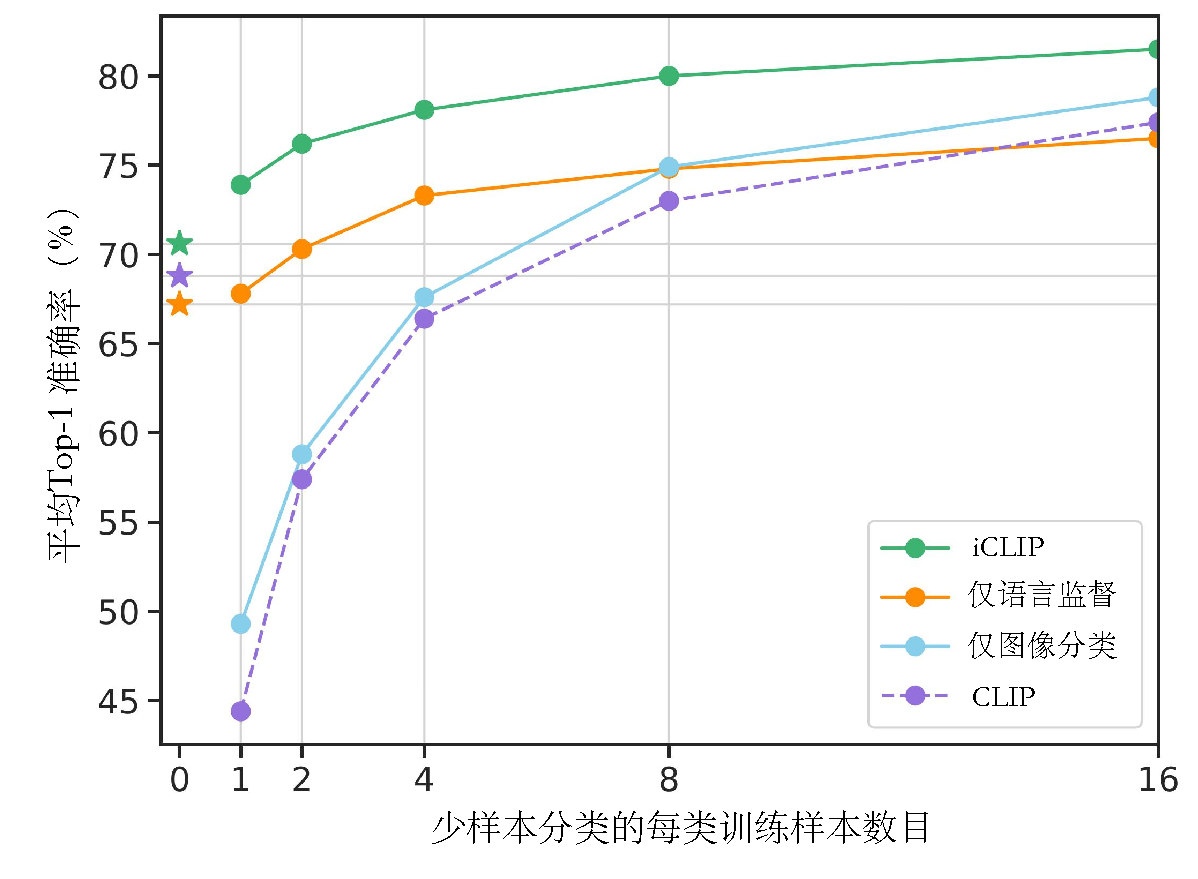
\includegraphics[width=0.8\linewidth]{figures/iclip-fewshot.pdf}
  \caption{iCLIP方法与不同方法在少样本图像识别任务微调上的性能比较}
  % todo: CLIP改为OpenAI CLIP
  % \todo{图4:与 Kornblith 12 数据集上小样本分类的 CLIP-ViT-B/16 的主要比较,展示了平均Top-1准确率。⋆表示零镜头性能。使用发布的模型再现了 CLIP 对少数镜头分类的结果。我们每个实验运行 3 次,并报告平均结果。}
  \label{fig:iclip-fewshot}
\end{figure}

\paragraph{少样本图像识别任务微调结果} 本组实验还比较了不同预训练方法在少样本图像识别任务上的微调性能,并选用Kornblith-12数据集作为训练和评测数据集。这项微调任务设置遵循了OpenAI CLIP工作的原始设置:在微调过程中固定视觉模型不变,只微调额外的类别分类器。
% 这组评测按照CLIP给出的设置实现:冻结视觉模型并增加一个额外的线性分类层以进行少样本微调。
如图\ref{fig:iclip-fewshot}所示,OpenAI CLIP工作在每个图像类别可训练样本数较少时的微调表现要弱于零样本图像识别任务评测结果,除非每个图像类别使用4个以上的训练样本。这是因为当少样本图像识别任务微调的训练样本数量有限时,随机初始化的类别分类器难以得到很好的训练,因此无法充分反映视觉表征中蕴含的语义信息。
基于前述利用对比学习方法重新表达图像分类任务的方法,在本组实验中直接微调经过预训练的语言模型作为类别分类器,而不是微调随机初始化的类别分类器。预训练过的语言模型能够为少样本图像识别任务微调提供良好的初始化,并缩小了语言-图像对比学习预训练阶段与少样本图像识别任务微调阶段之间的差异。

当每个图像类别只使用一个训练样本时,使用语言模型重参数化分类器权重的做法使得iCLIP方法达到73.9\%的平均Top-1准确率。相比于OpenAI CLIP工作高出29.5\%,也比iCLIP方法的零样本基线高出3.3\%,验证了其在少样本微调任务上的优势。当每个图像类别使用16个训练样本时,iCLIP方法的微调性能仍然比OpenAI CLIP工作要高4.1\%。
与单图像分类方法和单语言-图像对比学习方法的基线相比,iCLIP方法在单样本微调下的平均Top-1准确率分别提高了24.6\%和6.1\%,并在16个训练样本的设置中依然保持2.7\%和5.0\%的性能提升。

\begin{table}
  \centering
  % \addtolength{\tabcolsep}{-2.0pt}
    \caption{iCLIP方法与不同方法在下游视觉任务上的微调性能比较}
    %IN-22K和Laion-400M数据组合上的消融研究。我们在 ImageNet 数据集 (IN-1K [8] 和 IN-S [56])上评测模型,并在 Kornblith-12 数据集基准 [27] 上评测零样本评测。在 Kornblith-12 数据集上进行了小样本学习和对三个下游任务的微调,以评测iCLIP的迁移能力。$^\ddag$表示使用公开的模型权重进行测试。}
  \begin{tabular}{lccc}
  % method | visual encoder arch | image numbers# | IN-1K | IN-S | 12-zero | 12-four-shot | ADE | LVIS | K400
    \toprule
    \multicolumn{1}{c}{} & \multicolumn{1}{c}{图像语义分割} & \multicolumn{1}{c}{长尾类别物体检测} & \multicolumn{1}{c}{视频动作识别}\\
    % \cmidrule(lr){1-1} \cmidrule(lr){2-4}
    \midrule
  方法 & mIoU得分 & 检测框mAP得分 & Top-1准确率(\%)\\
    % \cmidrule(lr){1-1} \cmidrule(lr){2-4}
    \midrule
    仅图像分类方法 & 52.1 & 35.9 & 82.7 \\
    仅对比学习方法 & 52.0 & 36.6 & 82.3 \\
    iCLIP &\textbf{52.6} & \textbf{37.9} & \textbf{83.1} \\
    \bottomrule
  \end{tabular}

  \label{tab:iclip-overall-transfer}
\end{table}

\paragraph{在其他视觉下游任务上的微调结果} 本节对比了不同方法在其他视觉下游任务上的微调效果。如表\ref{tab:iclip-overall-transfer}所示,与仅使用图像分类方法的基线相比,iCLIP方法在图像语义分割、长尾类别物体检测和视频动作识别任务上分别提升了0.5的mIoU得分、2.0的检测框mAP得分和0.4\%的Top-1准确率。与仅使用对比学习方法的基线相比,iCLIP方法在三项视觉任务微调上也分别有0.6、1.3和0.8\%的提升。这些结果表明iCLIP方法获得的视觉表征具有更强的泛化能力。


\section{总结}
\label{sec:iclip-summary}
% 我们的贡献总结如下:
% ・我们将图像分类和对比语言 - 图像预训练这两个重要的视觉任务合并到一个框架中。
% ・我们发现原始图像分类公式可以适应 CLIP 方法,而性能几乎没有下降。根据这一发现,我们提出了一种有效融合方法,其中两个任务共享相同的文本编码器和相同的分类器类型,其有效性在基准测试中得到了广泛验证。
% ・我们提出了一种简单而有效的方法,将知识库引入图像分类中,解决了原始短图像名称的歧义和多义问题,并进一步弥合了类和替代文本之间的差距。它还首次展示了将知识库应用于计算机视觉问题。
% 背景+motivation
语言-图像对比学习方法通过对比学习框架在图文对数据中寻找正负样本对驱动模型预训练,并扩展到大规模互联网图文对数据。
但是这些图文对数据中存在大量标注噪声,影响了视觉表征与语言表征的对齐效果。

% 解决方案和发现
本章提出利用已有的人工标注数据,如高质量图像分类数据作为互联网图文对数据的补充。为有效融合两种不同形式的数据源和对应的训练方法,本章提出iCLIP预训练方法。
iCLIP方法一方面从语言-图像对比学习方法的角度重新理解传统的图像分类方法,统一了两种方法的损失函数形式和分类器参数化方式,另一方面引入外部专家知识库增强图像类别语义信息,对齐了不同数据在标注信息语义丰富度上的差异,并减少了类别标签间的歧义。
% 引入已有经过人工标注的数据源进行增强,一方面扩展了数据来源和监督信号类别,另一方面也提高了数据整体信噪比,有利于数据利用效率的提升。特别地,本章以已有的图像分类数据为主要对象,经过对图像分类任务的解析与重构,发现该类任务可以从实例级语言监督任务的角度重新诠释和建模,且不会损害其原有的学习效率,因此使得其有机会与原先的基于实例级对比的联合预训练方法,也即CLIP,进行有效融合。
% 具体来说,为将传统的图像分类任务与基于实例级对比的联合预训练方法对齐,引入了三项调整内容:用余弦相似度统一损失函数,用语言模型统一监督信号建模,引入外部知识哭缩小标签信息粒度差距。
经过高质量图像分类数据增强后的语言-图像对比学习iCLIP方法在零样本开放集合图像识别任务和图文跨模态检索任务上取得明显性能提升,并在亿级图像的大规模训练数据上得到验证。
% 同时本章工作在三种不同的数据组合规模,从百万级到亿级图片上进行了验证,充分展示了该方法的数据可扩展性。

% 引入下一章
虽然iCLIP方法在语义分割、物体检测等下游视觉任务上的微调性能有所提升,但提升幅度相对有限。因此,下一章将深入研究语言-图像对比学习方法在细粒度视觉任务上的迁移任务,并提出相应的改进方案。